\documentclass[
   10pt,                               % corpo del font
   a4paper,                            % formato foglio (default A4)
   DIV=calc,                           % margini
   english,
   italian
   ]{scrreprt}

\usepackage[utf8]{inputenc}

%**************************************************************
% Importazione package
%************************************************************** 

\usepackage[english, italian]{babel}   % per scrivere in italiano e in inglese;
                                       % l'ultima lingua è predefinita

\usepackage{booktabs}                  % tabelle          

\usepackage{tabularx}                  % tabelle di larghezza prefissata                                    
\usepackage{longtable}                 % tabelle su più pagine                                        
\usepackage{ltxtable}                  % tabelle su più pagine e adattabili in larghezza

\usepackage{csquotes}                  % gestisce automaticamente i caratteri (")

\usepackage{epigraph}					   % per epigrafi

\usepackage{eurosym}                   % simbolo dell'euro

\usepackage{graphicx}                  % immagini

\usepackage{hyperref}                  % collegamenti ipertestuali

\usepackage{listings}                  % codici

\usepackage[dvipsnames]{xcolor}        % colori

\usepackage{booktabs}                  % tabelle                                       
\usepackage{tabularx}                  % tabelle di larghezza prefissata                                    
\usepackage{longtable}                 % tabelle su più pagine                                        
\usepackage{ltxtable}                  % tabelle su più pagine e adattabili in larghezza

\usepackage{float}                     % utile per forzare figure dopo del testo con [H]

\usepackage{svg}                       % package per l'utilizzo di immagini in svg

\usepackage{caption}                   % package per gestire meglio le captions

\usepackage[
   toc,                                % glossario nella table of contents
   acronym                             % glossario di tipo acronym
   ]{glossaries}                       % glossario
\makeglossaries{}

%\usepackage[backend=biber,style=verbose-ibid,hyperref,backref]{biblatex}
                                       % eccellente pacchetto per la bibliografia; 
                                       % produce uno stile di citazione autore-anno; 
                                       % lo stile "numeric-comp" produce riferimenti numerici
                                       % per includerlo nel documento bisogna:
                                       % 1. compilare una prima volta tesi.tex;
                                       % 2. eseguire: biber tesi
                                       % 3. compilare ancora tesi.tex.

%**************************************************************
% file contenente le impostazioni della tesi
%**************************************************************

%**************************************************************
% Impostazioni KOMA Script
%**************************************************************

% Margini
\KOMAoptions{DIV=14}
\addtokomafont{disposition}{\rmfamily}
\KOMAoptions{fontsize=11pt}


%**************************************************************
% Comandi custom
%**************************************************************

% Autore
\newcommand{\myName}{Filippo Berto}                                    
\newcommand{\myTitle}{Sviluppo di una piattaforma di video streaming per l'assistenza remota tramite dispositivi wearable}

% Tipo di tesi                   
\newcommand{\myDegree}{Tesi di laurea triennale}

% Università             
\newcommand{\myUni}{Università degli Studi di Padova}

% Facoltà       
\newcommand{\myFaculty}{Corso di Laurea in Informatica}

% Dipartimento
\newcommand{\myDepartment}{Dipartimento di Matematica `Tullio Levi-Civita`}

% Titolo del relatore
\newcommand{\profTitle}{Prof.}

% Relatore
\newcommand{\myProf}{Tullio Vardanega}

% Luogo
\newcommand{\myLocation}{Padova}

% Anno accademico
\newcommand{\myAA}{2016--2017}

% Data discussione
\newcommand{\myTime}{Settembre 2017} %TODO: check solo mese

% Nome azienda
\newcommand{\nomeAzienda}{Vision Lab Apps}

% Nome azienda commerciale
\newcommand{\nomeAziendaComm}{Vision Lab Apps S.r.l.}

%**************************************************************
% Parole in Inglese
%**************************************************************

% Comando per parole in inglese: aggiunge emph e imposta la lingua
\newcommand{\engl}[1]{\emph{\foreignlanguage{english}{#1}}}

%**************************************************************
% Impostazioni di biblatex %TODO: check
%**************************************************************

%\bibliography{bibliografia} % database di biblatex 

%\defbibheading{bibliography} {
%    \cleardoublepage{}
%    \phantomsection{}
%    \addcontentsline{toc}{chapter}{\bibname}
%    \chapter*{\bibname\markboth{\bibname}{\bibname}}
%}

%\setlength\bibitemsep{1.5\itemsep} % spazio tra entry

%\DeclareBibliographyCategory{opere}
%\DeclareBibliographyCategory{web}

%\addtocategory{opere}{womak:lean-thinking}
%\addtocategory{web}{site:agile-manifesto}

%\defbibheading{opere}{\section*{Riferimenti bibliografici}}
%\defbibheading{web}{\section*{Siti Web consultati}}


%**************************************************************
% Impostazioni di glossaries
%**************************************************************
%**************************************************************
% Glossario
%**************************************************************
\newglossaryentry{AWS}
{
    name={AWS},
    description={Amazon Web Services (AWS) è una collezione di servizi di cloud computing on demand offerta da Amazon},
    first={Amazon Web Services (AWS)},
    long={Amazon Web Services}
}

\newglossaryentry{VPS}
{
    name={VPS},
    description={Un Virtual Private Server (VPS) è un'istanza di un sistema che viene eseguito in un ambiente virtuale},
    first={Virtual Private Server (VPS)},
    long={Virtual Private Server}
}

\newglossaryentry{IoT}
{
    name={IoT},
    description={Per Internet of Things (IoT) ci si riferisce all'estensione di Internet agli oggetti comuni, che diventano intelligenti e comunicano dati su se stessi e sul mondo che li circonda e allo stesso tempo accedere ad informazioni altrove nella rete},
    first={IoT},
    long={Internet of Things}
}

\newglossaryentry{wearable}
{
    name={Wearable},
    text={wearable},
    description={Si dice wearable un dispositivo elettronico indossabile on impiantabile. In generale questi dispositivi offrono delle funzionalità di notifica legate agli smartphone oppure contengono sensori per la rilevazione di attività fisica e sono un esempio di dispositivo \gls{IoT}}
}

\newglossaryentry{SEO}
{
    name={SEO},
    description={Si definisce Search Engine Optimization (SEO) l'attività di ottimizzazione dei contenuti di una pagina web per l'indicizzazione da parte dei motori di ricerca},
    first={SEO},
    long={Search Engine Optimization}
}

\newglossaryentry{CVS}
{
    name={CVS},
    description={É detto Concurrent Versioning System (CVS) un software che implementa un sistema di controllo di versione. Il sistema mantiene organizzati i cambiamenti fatti ad un certo numero di file e permette a molti sviluppatori di collaborare accedendo alle stesse risorse},
    first={CVS},
    long={Concurrent Versioning System}
} % database di termini
\makeglossaries{}

\begin{document}
   

%**************************************************************
% Parte iniziale
%**************************************************************

%**************************************************************
% Frontespizio 
%**************************************************************
\begin{titlepage}

\begin{center}

\begin{LARGE}
\textbf{\myUni}\\
\end{LARGE}

\vspace{10pt}

\begin{Large}
\textsc{\myDepartment}\\
\end{Large}

\vspace{10pt}

\begin{large}
\textsc{\myFaculty}\\
\end{large}

\vspace{30pt}

\begin{figure}[htbp]
\begin{center}
\includegraphics[height=6cm]{immagini/logo-unipd}
\end{center}
\end{figure}

\vspace{10pt} 

\begin{LARGE}
\begin{center}
\textbf{\myTitle}\\
\end{center}
\end{LARGE}

\vspace{10pt} 

\begin{Large}
\textsl{\myDegree}\\
\end{Large}

\vspace{40pt} 

\begin{large}
\begin{flushleft}
\textit{Relatore}\\ 
\vspace{5pt} 
\profTitle{}\ \myProf{}
\end{flushleft}

\vspace{10pt} 

\begin{flushright}
\textit{Laureando}\\ 
\vspace{5pt} 
\myName{}
\end{flushright}
\end{large}

\vspace{110pt}

\line(1, 0){338} \\
\begin{normalsize}
\textsc{Anno Accademico \myAA}
\end{normalsize}

\end{center}
\end{titlepage}

%**************************************************************
% Colophon
%**************************************************************
\clearpage
\phantomsection{}
\thispagestyle{empty}

\hfill

\vfill

\noindent\myName: \textit{\myTitle,}
\myDegree,
\textcopyright\ \myTime.
%TODO: citazione + dedica a fondo pagina
%TODO: pagina bianca
%TODO: sommario
%TODO: Ringraziamenti
%**************************************************************
% Indici
%**************************************************************
\cleardoublepage{}
\setcounter{tocdepth}{2}
\tableofcontents
%\markboth{\contentsname}{\contentsname} 
\clearpage
\listoffigures
%\listoftables
\cleardoublepage{}

%**************************************************************
% Contenuti
%**************************************************************

%**************************************************************
% Capitolo 1 - Introduzione
%**************************************************************
\chapter{Introduzione}
Lorem ipsum dolor sit amet, consectetur adipiscing elit. Morbi accumsan risus augue, vitae mattis arcu euismod at. Curabitur orci magna, volutpat quis est ut, suscipit ullamcorper velit. Cras et pulvinar est, et porta diam. Nam lobortis, justo eget posuere laoreet, felis ante condimentum turpis, ut semper nisi arcu non dui. Curabitur ut fringilla ligula. Phasellus cursus placerat auctor. Suspendisse vehicula sagittis laoreet. Duis dignissim nisi feugiat, consectetur leo ac, pellentesque sem. Vivamus vitae nulla eros. Duis vehicula enim sed elementum sagittis. Pellentesque id vehicula ipsum. Suspendisse maximus quis ligula eget malesuada. Lorem ipsum dolor sit amet, consectetur adipiscing elit.

Donec cursus urna nulla, ut interdum neque vulputate in. Curabitur sed dapibus enim. Integer felis ex, commodo eu aliquet id, venenatis sed diam. Duis ut velit erat. Quisque risus enim, egestas eu feugiat dictum, facilisis a sem. Aenean non est lorem. Proin sed cursus felis. Maecenas tincidunt libero tortor, condimentum tincidunt ligula suscipit facilisis. Duis dapibus finibus massa, quis pretium urna fringilla eu. Sed at nisl erat. Vestibulum quis nulla sit amet neque vehicula ultricies eu quis dolor. Nullam sit amet lacus dolor. Aliquam faucibus sed diam id vulputate.

Curabitur orci odio, gravida vitae tempor id, tincidunt at metus. Morbi aliquet tellus pharetra mauris convallis, in mattis diam vestibulum. Donec nec fermentum tortor, vel convallis est. Nullam sed nisl nisi. Duis id eros fermentum, dignissim massa a, bibendum metus. Sed ut convallis urna. Cras laoreet turpis ut erat pretium, et auctor est pellentesque. Quisque malesuada, dolor quis dictum feugiat, erat lacus sodales purus, eget vestibulum leo sem nec libero. Quisque gravida porttitor dui dignissim scelerisque. Donec in mollis ipsum, a varius lacus.

Sed quis pellentesque felis. Duis mollis mauris orci, sed pharetra arcu ultricies vitae. Mauris tempus dignissim ex. Ut lobortis fringilla nibh, rhoncus eleifend nisi sollicitudin sit amet. Sed at gravida nisi. Proin semper dolor eu venenatis sagittis. Maecenas maximus condimentum venenatis. Fusce nulla sem, consectetur vitae auctor imperdiet, vehicula quis nibh. Mauris magna metus, finibus luctus tempus sed, volutpat at ipsum. Aliquam vitae est a ligula pretium dignissim. Donec at tincidunt nibh, quis varius felis. Fusce eros eros, fermentum non pretium in, scelerisque a augue. Vestibulum dictum ipsum at tincidunt pretium. Mauris nisl felis, luctus non arcu eget, congue aliquam odio.

Vestibulum nisl massa, malesuada sed tortor nec, fringilla tincidunt metus. Nulla ut suscipit ex. Nulla non velit porta nulla venenatis sodales non vitae elit. Suspendisse rhoncus tincidunt dictum. In lorem tellus, facilisis vel efficitur vitae, pellentesque et elit. Sed tortor sem, ornare non ornare eu, molestie at risus. Nunc varius placerat consequat. Nunc eget ullamcorper turpis. Morbi dui nibh, consectetur at pharetra sed, tempus a ligula. Duis blandit dui lorem, in blandit ex consectetur nec.

Vivamus bibendum magna in fringilla faucibus. Etiam tincidunt nunc a sapien malesuada, quis mattis nisi venenatis. Nulla porta dapibus leo, in vehicula lacus aliquet ac. Sed urna tellus, feugiat non tellus a, varius vestibulum neque. Nullam arcu lorem, pharetra eu efficitur a, lobortis in odio. Pellentesque mattis vel ipsum non cursus. Sed accumsan ex nec sem dignissim malesuada. Duis luctus, purus sed pellentesque efficitur, dui ligula varius orci, quis maximus massa quam sed odio. Proin nunc purus, faucibus eget nulla lacinia, bibendum semper sapien. Integer a nunc at ligula tempor tempus. Sed sit amet ex quis nisi placerat pellentesque nec id mauris. Donec malesuada ac odio eget malesuada. Integer vulputate pulvinar eros, at cursus ante. Nunc at faucibus velit. Class aptent taciti sociosqu ad litora torquent per conubia nostra, per inceptos himenaeos.

Donec mollis lacinia leo, at ultrices leo accumsan at. Donec eu ipsum orci. Sed lacus nibh, vulputate vitae euismod nec, semper eu erat. Vestibulum vel tincidunt ligula. Aliquam aliquam venenatis lorem, at consequat magna hendrerit non. Nunc quis elit eros. Aenean volutpat euismod lacus sed mollis. Morbi urna nibh, lacinia vel hendrerit et, mollis porta nisi. Etiam dignissim molestie erat in iaculis. Donec ac ante ex. Ut quis augue et odio placerat feugiat non a ante. Ut urna mauris, dapibus ac tincidunt id, eleifend sed magna. Nam ut tortor id leo pretium aliquam sit amet ut mauris. Suspendisse tempor eros ligula, quis convallis purus sollicitudin malesuada. Proin in tincidunt arcu. Ut faucibus erat eget eros porta, ut consectetur nulla scelerisque.

Ut accumsan est et ipsum consectetur scelerisque. Integer consectetur dolor tellus, sed aliquet nulla gravida at. Vestibulum mattis sollicitudin enim non placerat. Morbi sit amet elementum quam. Fusce molestie nisl ut odio faucibus, nec condimentum mi elementum. Maecenas non nibh feugiat, facilisis arcu vitae, molestie quam. Ut in diam tellus. Nullam sagittis nisi in porta tempus. Phasellus egestas, enim non consectetur luctus, erat ligula scelerisque felis, et sollicitudin tortor ex a tellus. Nulla vel imperdiet tellus. Quisque id semper augue, ut vehicula dui. Etiam vestibulum massa sed ultricies dictum. Quisque eu est bibendum, pharetra tortor a, viverra purus. Aenean ultrices, mauris sed facilisis egestas, quam sem varius augue, mollis elementum tellus urna vitae eros.

Vestibulum a sodales tortor. In urna odio, auctor eu tristique et, ornare sit amet turpis. Sed auctor tempor nisi eget pretium. Duis aliquam sed orci eget vulputate. Nam dictum euismod dolor. Fusce eu convallis velit. Vivamus ac mi consectetur, pulvinar nibh quis, tincidunt odio. Suspendisse sit amet nunc in sapien feugiat ultrices eget scelerisque lorem. Aliquam sit amet dolor et lorem egestas viverra. Nunc faucibus pharetra diam, bibendum volutpat urna feugiat ultrices.

Phasellus non erat arcu. Pellentesque eu lectus dolor. Praesent porttitor rhoncus ipsum, vitae porttitor nisi luctus finibus. Nullam gravida, turpis elementum ultricies sodales, ante nibh bibendum risus, a consectetur sapien nisi porttitor urna. Aliquam dapibus leo placerat nibh dictum, in tempor lacus laoreet. Praesent mattis condimentum vestibulum. Vestibulum ornare massa quis nulla molestie imperdiet. Nullam ullamcorper lectus vel facilisis porta. Aliquam rutrum libero vel dolor venenatis, eget gravida neque efficitur. Nullam faucibus dapibus finibus. Aliquam et pretium nisi, a luctus libero. Sed a bibendum nulla, eget fermentum ligula. Duis pretium ligula eget nisl consectetur, in vehicula nisl porttitor. Proin vel sapien elementum, viverra libero at, tempus nisl. Duis euismod, sapien a egestas ornare, mauris nisi consequat erat, quis scelerisque est lacus quis arcu. Pellentesque id tortor varius, tempus nulla at, molestie eros.            % Introduzione - L'azienda
%**************************************************************
% Capitolo 2 - PERCHÉ - Scelta dello stage e rapporto con l'azienda
%**************************************************************
\chapter{Scelta dello stage e rapporto con l'azienda}
%TODO: introduzione capitolo

\section{Lo stage per l'azienda}

   \subsection{Necessità dell'azienda}
   \nomeAzienda{} sta sviluppando un sistema di videoconferenza per assistenza remota da applicare ai lavori specialistici e all'interno di aziende manifatturiere. Il sistema è pensato per aiutare un lavoratore inesperto, in situazioni difficili, facendolo guidare da una persona con le conoscenze adeguate a svolgere tali mansioni. Per rendere l'esperienza pratica funzionale, l'azienda ha pensato di utilizzare dei visori per la realtà aumentata, concentrandosi particolarmente sui Google Glass. L'utente esperto dovrà essere in grado di vedere in tempo reale quello che l'altro vede, tramite una videocamera integrata negli occhiali, e di mostrargli dati ed indicazioni su quello che deve fare, tramite il display integrato. Per realizzare tale progetto, \nomeAzienda{} necessita di un'intera piattaforma di streaming, che sta realizzando a componenti nel corso del tempo.
   \begin{figure}[H]
      \begin{center}
         
\includegraphics[width=16.5cm,keepaspectratio]{immagini/erastreaming-schema}
      \end{center}
      \caption{Schema generale del funzionamento della piattaforma di streaming}
   \end{figure}
   Il sistema che l'azienda vuole costruire è composto da tre elementi fondamentali, il client dell'utente sul campo, il sistema di relay e il client dell'utente esperto. Il primo è realizzato con uno smartphone Android e un paio di Google Glass; permetterà di registrare audio e video, inviati al sistema di relay tramite la rete del telefono, e di ricevere audio, video o messaggi di testo, inviati dal secondo client. Il client dell'utente esperto deve permettere di visualizzare e ascoltare i dati ricevuti e di poter rispondere con dati simili, per indicare al primo utente le azioni da compiere. Infine, il sistema di relay è composta da due elementi, un cluster di server di relay e un server amministratore; il primo è quello che si occupa del reinvio dei messaggi e della continuità della trasmissione tra i client connessi, mentre il secondo è adibito alla gestione dei canali, dell'autenticazione degli utenti e del bilanciamento del carico tra i nodi di relay.
   \\
   \nomeAzienda{} ha già realizzato un prototipo di client Android del servizio e, dopo test di trasmissione interni al dispositivo, si sta preparando per il passaggio alla comunicazione tra due dispositivi connessi ad una rete locale. Successivamente l'azienda provvederà a creare un sistema di amministrazione sfruttando Firebase e il suo servizio di autenticazione sicura.
   \begin{figure}[H]
      \begin{center}
         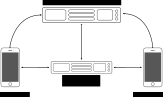
\includegraphics[width=12cm,keepaspectratio]{immagini/erastreaming-schema-attuale}
      \end{center}
      \caption{Schema delle componenti in fase di sviluppo}
   \end{figure}
   L'Obiettivo dello stage è quello di sviluppare il software del server di relay, necessario per far comunicare i due client. Il server deve permettere ai due dispositivi di inviarsi messaggi di qualsiasi tipo, senza che uno conosca l'indirizzo di rete dell'altro, e di gestire i canali e gli utenti tramite un API amministratore.
   
   \subsection{Risultati degli stage precedenti e seguito degli stagisti nell'azienda}
   \nomeAzienda{} ha deciso anche quest'anno di partecipare all'evento ``StageIt'', organizzato da Confindustria Padova in collaborazione con l'Università degli Studi di Padova, e di proporre agli studenti un tirocinio interno all'azienda. L'impresa è alla ricerca di neolaureati per arricchire il proprio team di sviluppatori, dato il recente aumento di clienti e la conseguente espansione.
   \nomeAzienda{} è, in particolare, interessata a studenti che sono appassionati di nuove tecnologie e che hanno interesse a imparare nuove tecniche e a farne conoscere di nuove all'azienda stessa.
   L'impresa ha già organizzato tirocini con altri studenti negli anni precedenti, ottenuto risultati soddisfacenti, tanto che molti degli ex stagisti sono stati assunti dall'azienda.

\section{Rapporto con il mio stage e con l'azienda}
   \subsection{Ambiti di interesse}
   Al momento della ricerca di uno stage ho prestato particolare attenzione alle aziende che proponevano un percorso legato ai miei interessi di studio. In particolare cercavo tirocini il cui argomento fosse compreso tra i seguenti:
   \begin{itemize}
      \item{Sicurezza;}
      \item{Sistemi ad alta concorrenza;}
      \item{Dispositivi IoT;}
      \item{Sistemi virtualizzati;}
      \item{Servizi cloud;}
      \item{DevOps;}
      \item{Sistemi multimediali.}
   \end{itemize}

   \subsection{Proposte di stage ricevute}
   Nei giorni immediatamente seguenti all'evento StageIt sono stato contattato da alcune aziende presenti delle quali ho selezionato le proposte che più mi parevano interessanti.
   \\
   Uno dei progetti proposti consisteva in un sistema di controllo di risorse e consumi di sistemi virtualizzati tramite \gls{Docker}: il software doveva fornire una chiara visione dello stato di ciascun servizio e riportare eventuali anomalie. Lo stage mi avrebbe permesso di conoscere meglio l'utilizzo di Docker, specialmente in un contesto DevOps, e di imparare nuove tecnologie di gestione di gruppi di contenitori, in particolare Kubernetes; fondamentali in un contesto di continuous deployment e continuous release. Le conoscenze che mi avrebbe fornito questo tirocinio erano di mio grande interesse, ma, sfortunatamente, non sono stato scelto, tra i possibili candidati.
   \\
   Un altro stage riguardava la realizzazione di un software in grado di unificare la grande mole di dati dell'azienda, sparsa tra diversi sistemi aziendali legacy e i \gls{CMS} dei loro clienti. Il prodotto avrebbe dovuto raccogliere i dati, salvarli in un formato comune, facilmente accessibile, e aggiornare i sistemi in caso di modifiche. L'utilità di un software del genere è molto elevata per un'azienda, ma il prodotto in sé consiste in un certo numero di adattatori per ciascuna delle fonti di dati, e non mi avrebbe fornito particolari conoscenze aggiuntive, rispetto a quelle che già possedevo.
   \\
   Un altro progetto proposto, invece, prevedeva la realizzazione di un sistema per la gestione delle traduzioni dei testi di un catalogo prodotti, consentendo visualizzazione, modifica e la ricerca di testi ripetuti tramite Elasticsearch, per l'ottimizzazione delle spese di traduzione. Elasticsearch è un motore di analisi del testo il cui utilizzo si sta diffondendo molto in fretta, ma lo stage non comprendeva lo studio del suo funzionamento. Il prodotto avrebbe anche dovuto generare una serie di informazioni, come un preventivo dei costi di traduzione e una lista di frequenza di certe espressioni.
   \\
   Un ulteriore tirocinio prevedeva un progetto sperimentale per lo spostamento di un software di rendering \gls{CAD} per \gls{TAC} da un sistema locale a uno client-server, con elaborazione dei dati su server virtualizzati. Il video elaborato sarebbe poi stato servito a un \gls{thin client}; alleggerendolo del carico di computazione del render. Il progetto comportava la scomposizione del software proprietario dell'azienda, lo studio di una soluzione di virtualizzazione e l'integrazione con una libreria per la trasmissione dei dati. Sebbene lo stage proposto toccasse molti e vari ambiti, si sarebbe concentrato solo in una parte del progetto, prevedendo la continuazione da parte dello studente dopo la laurea. Considerata la mia scelta di continuare i miei studi, non ho potuto accettare la proposta dell'azienda.

   \subsection{Scelta dello stage}
   %TODO: espandere sezione
   Al momento della scelta di quale stage accettare, tra quelli proposti, ho preferito optare per quello che proponeva argomenti per me più nuovi e meno conosciuti, che producesse, quindi, il migliore valore aggiunto per mie competenze.
   Ho scelto il progetto di \nomeAzienda{} perché ho trovato il campo di cui si occupa interessante e le mie conoscenze sull'argomento erano solo marginali. Inoltre una più approfondita conoscenza di sistemi ad alta concorrenza, come può essere un servizio di streaming, è applicabile a molti altri campi, come sistemi cloud distribuiti e dispositivi IoT.

   \subsection{Scelta dell'azienda}
   Durante la scelta dello stage ho considerato marginale l'aspetto del futuro in azienda, dato che la mia scelta di continuare a studiare per la laurea magistrale è incompatibile con un lavoro a tempo pieno. Il mio interesse più grande era quello di poter collaborare con persone più esperte di me per imparare cose nuove; per questo motivo mi sono accertato che durante il tirocinio avrei potuto interagire con molte figure dell'azienda che si occupano di sviluppo.
   \\
   Un altro importante fattore che ho deciso di ignorare è stata la distanza dell'azienda dalla mia residenza: ho preferito dare più importanza all'esperienza dello stage in sé rispetto alla comodità di spostamento.

\section{Obiettivi del progetto di tirocinio}
All'inizio del progetto di tirocinio sono stati definiti gli obiettivi, distinti poi in obbligatori e desiderabili, e i vincoli tecnologici ai quali ho dovuto attenermi. Ne segue una lista dei fondamentali.

   \subsection{Obiettivi obbligatori}
   \begin{itemize}
      \item{Studio dei formati video e dei protocolli di rete per le trasmissioni video in real-time e on-demand;}
      \item{Studio dell'architettura di rete di un servizio di streaming;}
      \item{Sviluppo di un applicativo server per il relay di messaggi tra i suoi client.}
   \end{itemize}

   \subsection{Obiettivi desiderabili}
   \begin{itemize}
      \item{Studio delle problematiche della trasmissione di dati in mobilità;}
      \item{Sistema di autenticazione dei client e organizzazione a canali delle trasmissioni;}
      \item{Studio di possibili utilizzi della tecnologia Blockchain nel campo dello streaming.}
   \end{itemize}

   \subsection{Vincoli tecnologici}
   Mi è stato richiesto di utilizzare Java come linguaggio di programmazione, per consentire una più veloce integrazione con il client Android. Inoltre, data la struttura a servizi della piattaforma, ho dovuto utilizzare un server Java come base del prodotto.

\section{Pianificazione del lavoro}
La pianificazione del progetto è stata eseguita in accordo con il tutor interno. Nella prima settimana ho avuto modo di studiare gli strumenti, i formati e i protocolli necessari alle funzioni della piattaforma, stilando una relazione sullo stato dell'arte. Ho, poi, proseguito con l'analisi delle funzionalità richieste e la definizione di requisiti e casi d'uso. Ho impiegato la terza settimana nella progettazione del servizio e della componente server, per poi procedere le due settimane successive alla sua realizzazione. Per garantire una buona qualità del codice, ho dedicato una settimana alla validazione, ai beta test e alla riformattazione. L'ultima settimana ho ultimato la documentazione del progetto e dei risultati ottenuti.
\begin{figure}[H]
   \begin{center}
      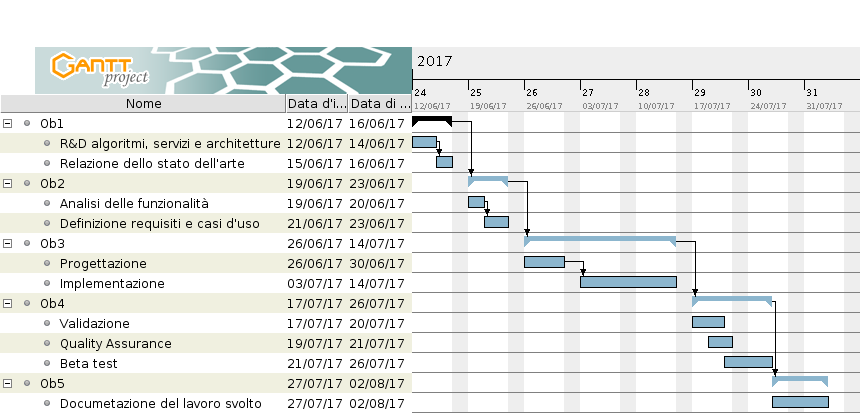
\includegraphics[height=8cm,width=15cm,keepaspectratio]{immagini/pianificazione-gantt}
      \caption{Diagramma di Gantt della pianificazione}
   \end{center}
\end{figure}

   \subsection{Strumenti utilizzati}
   Per ottenere buoni risultati durante la pianificazione \nomeAzienda{} utilizza GanttProject\footnote{Sito web del progetto GanttProject: \href{http://www.ganttproject.biz/}{www.ganttproject.biz}}, un software open-source per la realizzazione di diagrammi di \gls{Gantt} e \gls{PERT}. Il programma permette di costruire diagrammi con estrema facilità, gestendo scadenze, risorse, personale e dipendenze; inoltre permette di esportare il risultato in HTML o in formato PNG.\
            % Progetto di stage

\appendix                               
%\input{capitoli/capitolo-A}            % Appendice A

%**************************************************************
% Parte finale
%**************************************************************

\printglossary[toctitle=Glossario]{}
%**************************************************************
% Bibliografia
%**************************************************************

\cleardoublepage{}

\begin{thebibliography}{9}
   
   \bibitem{mobiledesktopusage}
      James Titcomb,
      \textit{Mobile web usage overtakes desktop for first time},\\
      \href{www.telegraph.co.uk/technology/2016/11/01/mobile-web-usage-overtakes-desktop-for-first-time}{www.telegraph.co.uk/technology/2016/11/01/mobile-web-usage-overtakes-desktop-for-first-time},\\
      The Telegraph,
      1 November 2016
   
   \end{thebibliography}

\end{document}
